\section{Methodology}
\label{headings}
\begin{figure*}[t]
    \centering
    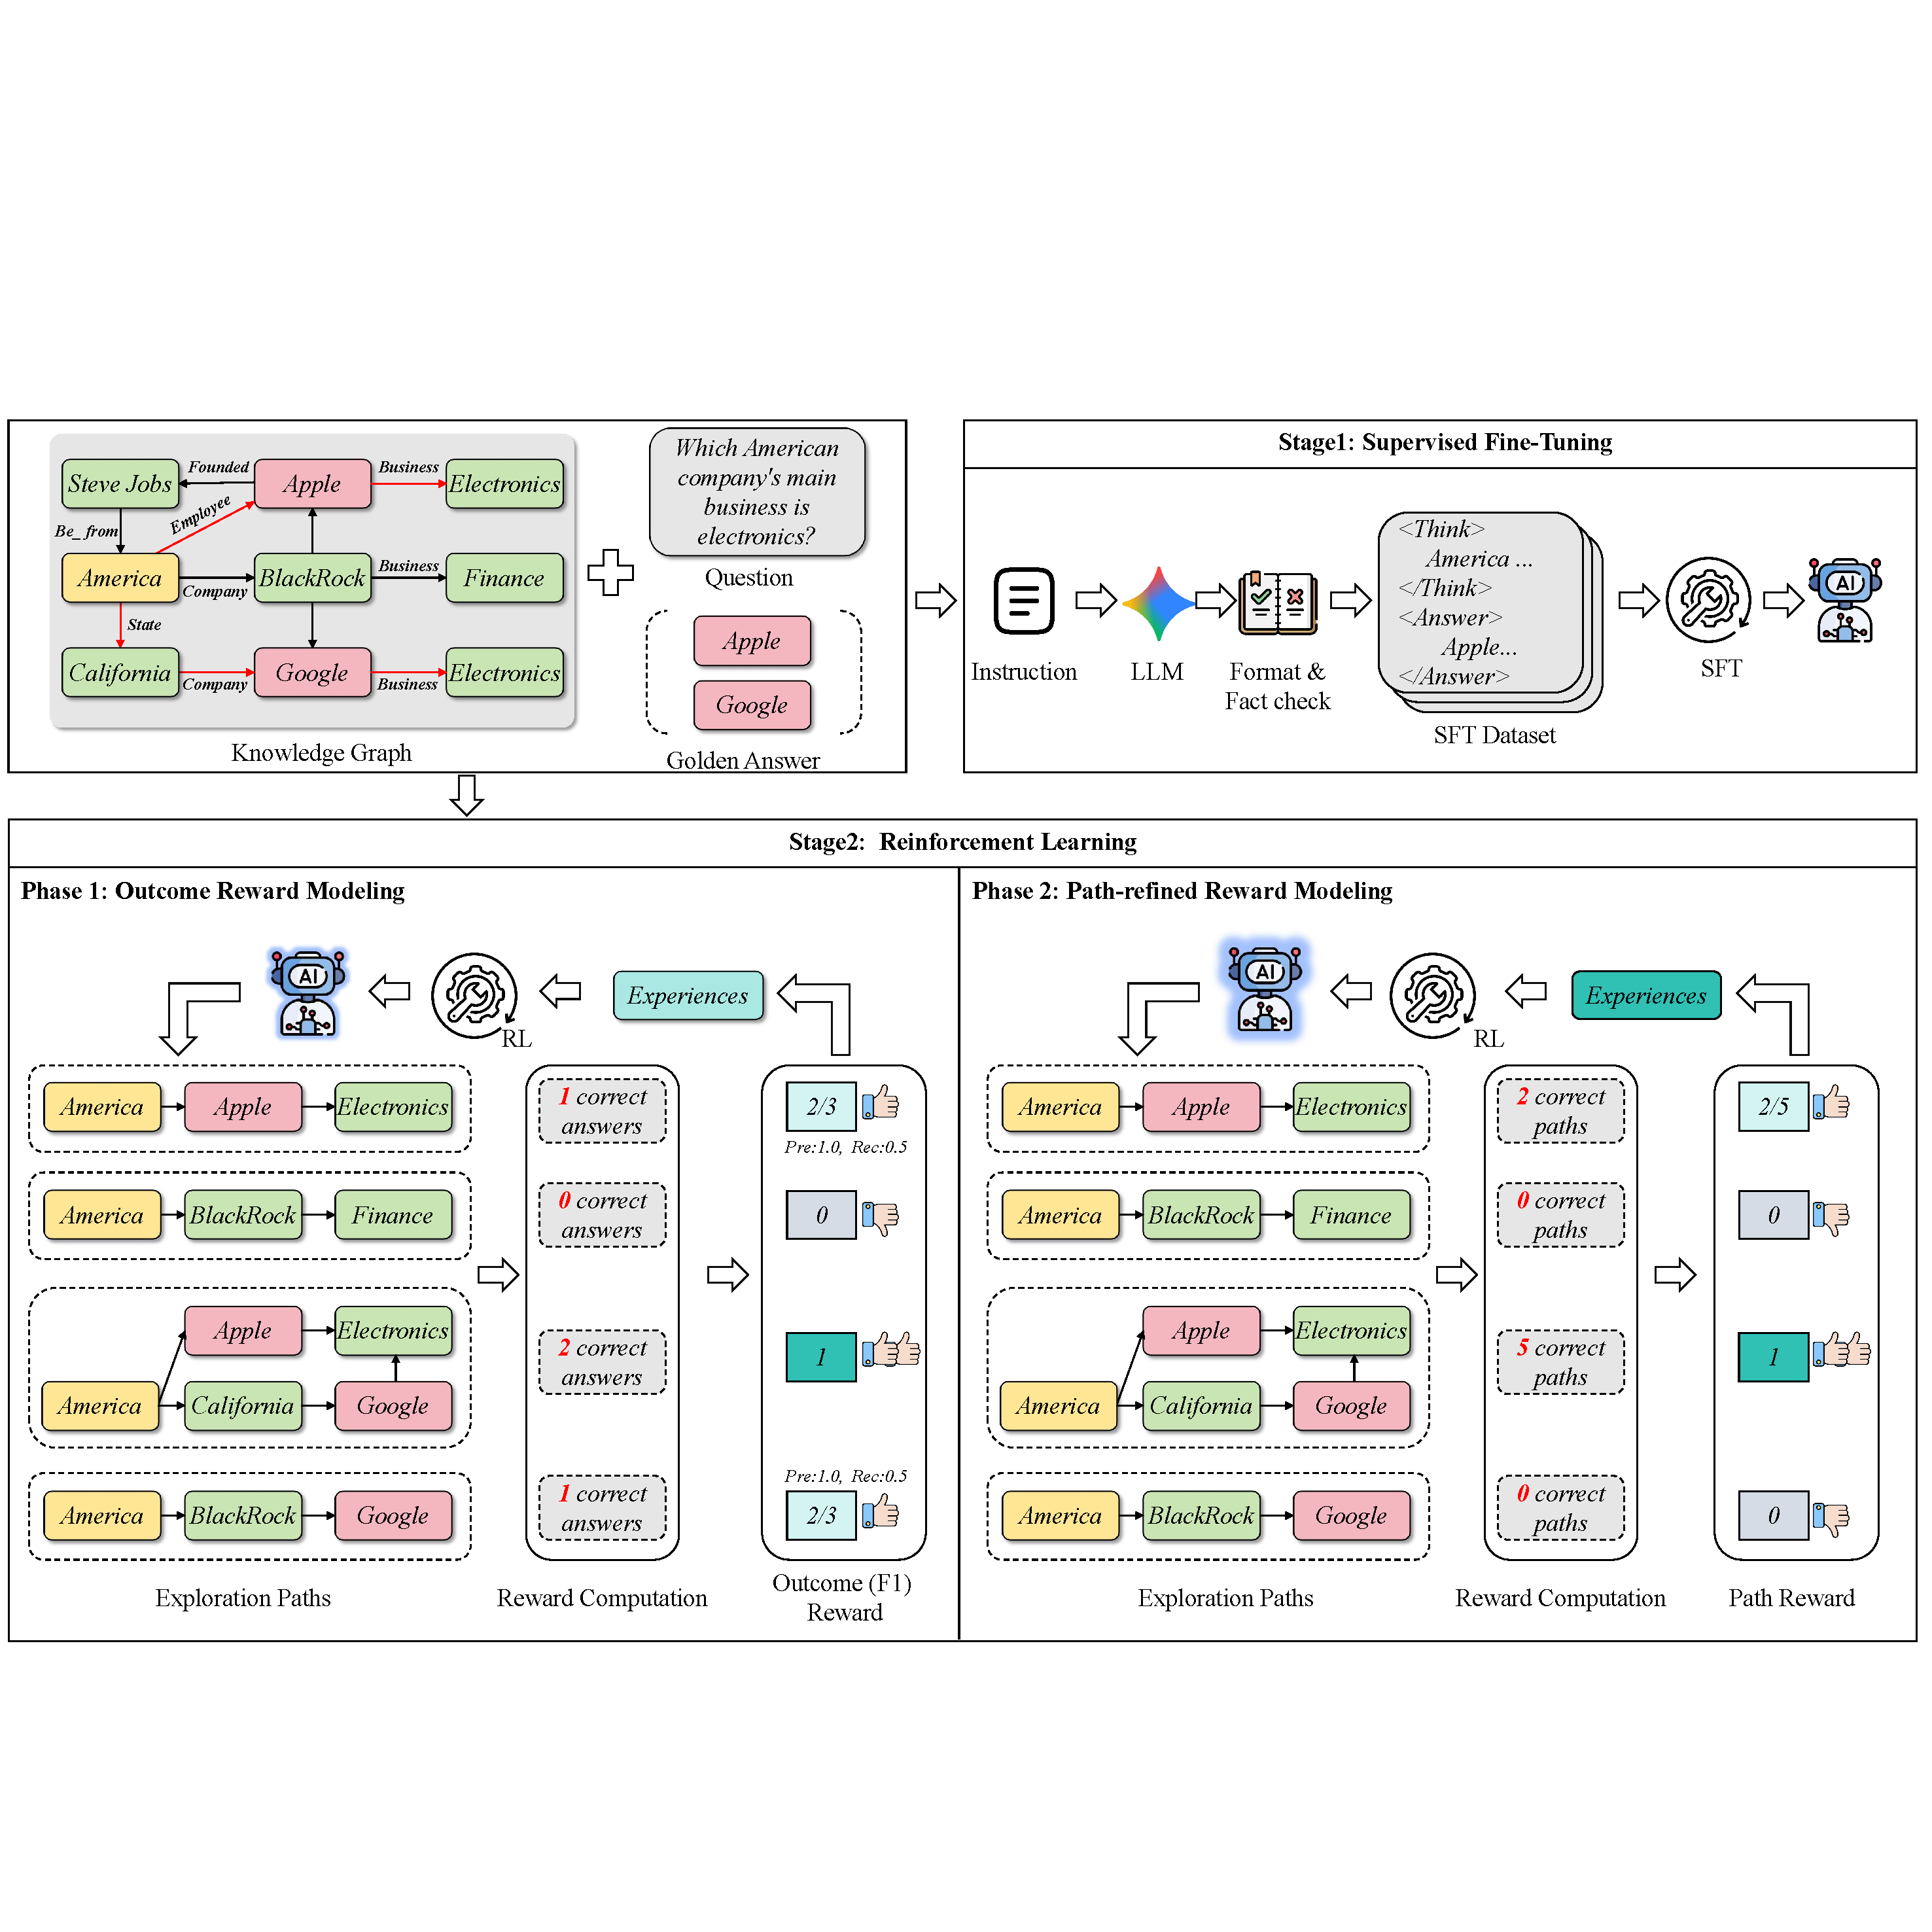
\includegraphics[width=.95\textwidth]{figures/methods.pdf}
    \caption{The overall framework of our approach. Red arrows in the knowledge graph stands for the golden reasoning paths of the given question.}
    \vspace{-7pt}
    \label{fig:framework}
\end{figure*}
In this section, we introduce our Explore-on-Graph (EOG) in detail, which consists of a Supervised Fine-Tuning (SFT) stage and a Reinforcement Learning (RL) stage.
To equip LLMs with the foundational ability for graph exploration, we introduce the SFT on knowledge graph reasoning tasks in Section \ref{subsec:longcot}.
To motivate the exploration of various reasoning paths and enhance its efficiency and meaningfulness, we introduce the RL with path-refined reward modeling in Section \ref{subsec:rl}.
The general framework of our approach is illustrated in Figure \ref{fig:framework}.


% The core objective of our method is to train a model, parameterized by $\theta$, to produce a high-quality output sequence $z$ by performing multi-step reasoning over a structed knowledge graph. Formally, given a set of inputs including a graph $\mathcal{G}$, a question $x$, and a starting entity $e_s$, the model learns to generate a sequence $z = (r, y)$ that maximizes a predefined quality objective.Our method can be formulated into three stages as detailed below.
% \subsection{Knowledge Graph Construction}
% Due to the limited input length of  language models and the substantial increase in training time as the input length grows, we opt to use a  language model to extract relevant triples from the  knowledge graph $\mathcal{G}$ that are related to the question.Given starting entities $e_s$ and a question $q$, we use a language model to extract entities related to the question from its three-hop neighbors. The triples $(h, r, t)$  formed by these entities and relations constitute the graph $\mathcal{G}_{\text{train}}$.

% \begin{equation}
% \mathcal{G}_{\text{train}} = \{ (h, r, t) \in \mathcal{G} \mid h, t \in \{e_s\} \cup \text{}_{\mathcal{M}_{\text{LM}}}(q, \mathcal{N}_3(e_s)) \}
% \end{equation}

% where $\text{Extract}_{\mathcal{M}_{\text{LM}}}$ denotes a language model-based function that extracts a set of relevant entities from the 3-hop neighborhood $\mathcal{N}_3(e_s)$ of the start entity $e_s$, conditioned on the question $q$.

\subsection{Supervised Fine-Tuning}
\label{subsec:longcot}
% Without establishing a solid foundation for the subsequent exploration phase, the reinforcement learning process would operate in an excessively vast and unstructured action space, leading to inefficient exploration, reward sparsity, and potentially misguided policy updates. 
% To mitigate these challenges, we introduce Long Chain-of-Thought Supervised Fine-tuning, which provides the model with structured, exemplary reasoning trajectories. 
% This approach not only equips the model with essential reasoning skills but also effectively constrains and guides the subsequent exploration, enabling more efficient and meaningful policy refinement.
Directly instructing the LLMs to explore KGs presents significant challenges, including an intractably large action space and extreme reward sparsity~\citep{xiong-etal-2017-deeppath,LinRX2018:MultiHopKG}, due to lack of prior knowledge.
To bridge this gap, CoT offers a pathway of structured reasoning demonstrations, by teaching LLMs the complex multi-step logic necessary for knowledge graph exploration~\citep{wu2024cotkr}.
Compared to short CoT, long CoT allows more comprehensive and in-depth reasoning by exploring a wider range of logical paths~\citep{chen2025towards}.
 % This approach explicitly trains LLMs to follow coherent reasoning paths that mirror the multi-step logic required for robust graph navigation.
Therefore,  we employ the long CoT Supervised Fine-Tuning paradigm to establish a foundation for the subsequent exploration phase, which consists of two parts: (1) constructing the long CoT reasoning dataset and (2) fine-tuning LLMs with the constructed dataset.
% Therefore, we employ the Long CoT SFT paradigm for the first stage of training, which consists of two parts: (1) constructing a Long CoT reasoning dataset on graphs via distillation in Section , and (2) training the model through SFT to acquire reasoning paradigm from this dataset.
 
% Moreover, by learning to imitate these correct reasoning paths, the LLM receives dense, step-by-step supervisory signals, which directly counteract the reward sparsity problem. 
% Through this supervised pre-training phase, the model acquires a strong capacity for structured reasoning, establishing an essential foundation for the subsequent exploration phase. In this phase, reinforcement learning can then effectively refine and diversify these learned pathways based on environmental feedback, rather than starting from unguided random exploration.
% To mitigate these challenges, we introduce Long Chain-of-Thought Supervised Fine-tuning, which provides LLMs with structured, exemplary reasoning trajectories. 
% This approach explicitly trains LLMs to follow coherent reasoning paths that mirror the multi-step logic required for robust graph navigation.

% By learning from demonstrations of structurally sound and factually accurate trajectories, the model acquires a strong capacity for structured reasoning, establishing an essential foundation for the subsequent exploration phase, where reinforcement learning can then effectively refine and diversify these learned pathways rather than starting from unguided random exploration.
% To enable the model to preliminarily possess the long cot capability for step-by-step reasoning on the graph, we employ the Long CoT Supervised Fine-Tuning paradigm for the first stage of training, which consists of two parts: (1) constructing a Long CoT reasoning dataset on graph via distillation and rejection sampling, and (2) training the model through SFT to acquire reasoning paradigm from this dataset.

\textbf{Long CoT Dataset Construction.} We carefully design the prompt to generate long CoT for graph reasoning, 
which requires the reasoning process to be structured, logical and to be aligned with KGs. The detailed prompt could be found in Figure \ref{fig:appendix_sft_prompt}.
Due to its advanced deep thinking capabilities, we select Gemini 2.5 Flash~\citep{comanici2025gemini} to perform knowledge distillation to generate long-chain reasoning thoughts and the final answers.
Given a knowledge graph $\mathcal{G}$ and a question $q$ as the query input, the generation sample from Gemini 2.5 Flash can be defined as the reasoning process $z$, which comprises both the reasoning paths (within ``$<think></think>$'' tags) and the final answers (within ``$<answer></answer>$'' tags).
% Then we introduce a strict filtering process where we retain only the samples that adhere to the structured format and feature a reasoning path and the corresponding answers aligned with the knowledge graph.
Then we incorporate additional rules to filter the reasoning process that is both structurally and factually correct.
Finally, the SFT dataset $\mathcal{D}_\textrm{CoT}$ is constructed, with high-quality long CoT reasoning processes.
% This rigorous pipeline ensures the creation of high-quality data for model training.

% constructed long CoT datasets for graph reasoning through the distillation processes from Gemini-2.5 Flash~\citep{comanici2025gemini},
% .followed by strict filtering. We kept only the samples that 1) followed the correct XML output format, 2) had a correct answer from the graph, formatted as a list, and 3) contained a reasoning process that started from the correct entity and used information from the graph. This ensures high-quality data for training the model.

% \subsubsection{Long CoT Dataset Construction}
% \label{subsubsec:longcotconstruction}
% To endow the model with long CoT capability for exploration on graphs, we developed an approach to construct a long CoT dataset by prompting Gemini-2.5 Flash with knowledge based question answering and applying rejection sampling to obtain data that only contains correct answers and conforms to our desired format.Each sample in the dataset follows this format:$(G, q, r, y,o)$,where G denotes the knowledge graph used for training and answer to any question is guaranteed to be among the entities within this knowledge graph,q is the knowledge based question which is multi-hop quenstion,r and y represents long chain-of-thought reasoning processes and structured answer formats,o encapsulates both the reasoning process and the final answer.Inspired by the principle of rejection sampling, we apply multiple filtering rounds to the samples, ensuring only well-structured samples with answers consistent with the standard answers are retained. The specific filtering criteria are as follows:

% \textbf{1.Format Check:}We first ensure that the generated answers must follow XML-like tags: \verb|<think>...</think> <answer>...</answer>|. If the format is not followed, we regenerate until it complies. Samples that cannot be successfully regenerated are subsequently discarded.

% \textbf{2.Answer Check:}First, we verify answer correctness and knowledge graph traceability by checking whether the generated answer exactly matches the gold standard and is an entity from the graph, ensuring high-quality samples.This guarantees high sample quality.Subsequently,we validate that the answer is formatted as a list structure, such as \verb|["openai", "claude"]|,which facilitates the subsequent computation of F1 scores in the RL training phase.

% \textbf{3.Reasoning Check:}The quality of the reasoning process is crucial for Long CoT capability. It is difficult to prompt the model to produce the desired Long CoT output. Therefore, we apply two criteria for data filtering: the reasoning process must begin by mentioning the \verb|begin_entity|, which ensures the model's starting point aligns with the question requirements. Additionally, the reasoning should utilize information from the graph, since the graph is guaranteed to contain the correct answer. This prevents the model from relying on its own knowledge to answer questions.

% The purpose of the three-dimensional quality checks is to support the subsequent RL training process. Only samples that pass all three checks are retained, ensuring that the SFT phase can endow the model with high-quality reasoning capabilities over structured knowledge graphs.

% % Meanwhile, our dataset contains multi-hop questions with varying hop counts and causal patterns, which ensures that the model can develop robust Long CoT capabilities across different numbers of hops or diverse causal patterns over structured knowledge graphs.

% In summary, the three-dimensional quality check filters samples to ensure that the supervised fine-tuning phase produces a model with reliable reasoning capabilities over structured knowledge graphs. Combined with the intrinsic diversity of hop counts and causal patterns in the dataset, we efficiently endow the model with robust long-chain reasoning abilities for knowledge graph question answering tasks.


% \subsubsection{Supervised Fine-Tuning}
% \label{subsubsec:sft}
\textbf{Supervised Fine-Tuning.}
Following dataset construction, we perform SFT to endow the model with structured long CoT reasoning capabilities. 
% Given a knowledge graph $\mathcal{G}$ and a question $q$ as input, the model is trained to generate a complete reasoning process $z$, which comprises both the reasoning path and the final answers. 
We introduce a standard language modeling objective:
% \begin{equation}
% \mathcal{L}_{\textrm{SFT}} = - \sum_{(\mathcal{G}_i, q_i, z_i) \in \mathcal{D}_\textrm{CoT}} \sum_{j=1}^{|z_i|} \log P(z_{i,j} | z_{i,<j}, \mathcal{G}_i, q_i; \theta),
% \end{equation}
\begin{equation}
\mathcal{L}_{\textrm{SFT}} = - \frac{1}{|\mathcal{D}_\textrm{CoT}|} \sum_{i=1}^{|\mathcal{D}_\textrm{CoT}|} \sum_{j=1}^{|z_i|} \log P(z_{i,j} | z_{i,<j}, \mathcal{G}_i, q_i; \theta),
\end{equation}
where $(\mathcal{G}_i, q_i, z_i) \in \mathcal{D}_\textrm{CoT}$ is the $i$-th sample in the long CoT dataset, $z_i$ represents the complete reasoning process for the $i$-th sample, $z_{i,j}$ is the $j$-th token of that sequence, and $\theta$ denotes the LLM parameters. 
% This training stage compels the model to not only derive the correct answer but also to articulate a step-by-step, verifiable reasoning process grounded in the provided knowledge graph.
Through this phase, the LLM acquires a strong capacity for structured reasoning, establishing an essential foundation for the subsequent exploration phase. Reinforcement Learning (RL) can then effectively refine and diversify these learned pathways based on environmental feedback, rather than starting from unguided random exploration.

\subsection{Reinforcement Learning}
\label{subsec:rl}
While the SFT equips the LLM with the ability to generate structured reasoning paths, 
its outputs are usually confined to the patterns observed in the training data,
potentially leading to suboptimal reasoning. 
% To discover a broader and more effective exploration space, we introduce exploration-oriented reinforcement learning (RL) with path-refined reward modeling in this stage.
% The goal of this stage is to incentivize LLMs to explore novel entities and relations within the knowledge graph.
To facilitate the discovery of a broader and more effective exploration space, we structure our reinforcement learning approach into two distinct phases.
Inspired by advances such as Deepseek-R1~\citep{deepseek-math}, 
firstly, we introduce the Group Relative Policy Optimization (GRPO) to optimize the exploration policy on KGs based on the correctness of the reasoning path's final answers in Section~\ref{subsubsec:grpo}.
Then we integrate a path-refined reward that provides additional signals to steer exploration toward more efficient and meaningful paths in Section~\ref{subsubsec:pathreward}.
% However, its drawback is insufficient exploration capability---the model only excels at the reasoning patterns present in the long CoT data and lacks the ability to generalize. 
% Inspired by advances such as Deepseek-R1~\cite{deepseek-math}, we introduced Group Relative Policy Optimization (GRPO) to optimize the exploring policy $\pi_\theta$ toward  


% train the post-SFT model with the aim of stimulating the model's exploring capability over structured knowledge graphs. 

% Compared to SFT, RL is more like trial-and-error learning, excels at exploring new strategies, and the model adjusts its strategy (model parameters) based on correctness (reward signal). Our entire task can be formulated as $z = f(\mathcal{G}, q, e, r_g)$, where $\mathcal{G}$ is the knowledge graph, $q$ is the question, $e$ is the starting entity, and $r_g$ is the pre-defined reasoning path.
\subsubsection{Reinforcement Learning with Outcome Reward}\label{subsubsec:grpo}
% To further enhance the model's reasoning and exploration capabilities, we apply Group Relative Policy Optimization (GRPO) to refine the post-SFT model. GRPO avoids the need for a learned value function by calculating relative advantages within a group of sampled trajectories.
In the first phase, we optimize the exploration policy $\pi_\theta$ for enhancing the discovery of correct answers via a GRPO-based and outcome-supervised reinforcement learning objective $\mathcal{J}_{\textrm{GRPO}}(\theta)$ .
Given the environment $(\mathcal{G}, q) \in \mathcal{D}_\textrm{GRPO}$, our LLM after the SFT stage could generate a group of $S$ candidate exploration processes $\left \{ p_i \right \} _{i=1}^{S} \subseteq \mathcal{P}_{(\mathcal{G}, q)}$, where each $p_i$ is $i$-th process sampled from the old policy $\pi_{\theta_{\textrm{old}}}$.
Similar to a reasoning process $z$, each $p$ contains both the exploration paths and the final answers with structured tags.
The policy model could be optimized by maximizing the following reinforcement learning objective $\mathcal{J}_{\textrm{GRPO}}(\theta)$:

% Given a state $s = (x, \mathcal{G})$, consisting of the input question and the knowledge graph, the policy from the previous iteration $\pi_{\text{old}}$, generates a group of $G$ candidate reasoning sequences $\{z_1, z_2, \dots, z_G\}$. The GRPO objective for updating the policy parameters from $\theta_{\text{old}}$ to $\theta$ is:

% \begin{align}
%     \mathcal{J}_{\textrm{GRPO}}(\theta) &= {\mathbb{E}_{[(\mathcal{G},q) \sim {\mathbb{P}(\mathcal{G},q ) |(\mathcal{G},q \in \mathcal{D}_\textrm{GRPO})},\left \{ p_i \right  \} _{i = 1}^{S} \sim \pi_{\theta_{\textrm{old}}}(\mathcal{P}_{(\mathcal{G}, q)}|p_i;\mathcal{G} )]}}  \\
%  &\frac{1}{S}\sum_{i=1}^{S}  \frac{1}{|p_i|} \sum_{t = 1}^{|p_i|}\left \{  \min \left[\left( \frac{\pi_{\theta}(p_{i,t} | q,\mathcal{G} ,p_{i< t})}{\pi_{\theta_{\text{old}}}(p_{i,t} | q,\mathcal{G} ,p_{i< t})} \hat{A}_i, \text{clip} \left( \frac{\pi_{\theta}(p_{i,t} | q,\mathcal{G} ,p_{i< t})}{\pi_{\theta_{\text{old}}}(p_{i,t} | q,\mathcal{G} ,p_{i< t})}, 1 - \epsilon, 1 + \epsilon \right) \hat{A}_i \right) \right] - \beta \mathbb{D}_{\text{KL}}(\pi_{\theta} || \pi_{\text{ref}})\right \}
% \end{align}
% \begin{equation} \label{eq:Grpo}
% \begin{split}
%     \mathcal{J}_{\textrm{GRPO}}(\theta) &= {\mathbb{E}_{[\mathcal{G},q \sim {\{\mathbb{P}(\mathcal{G},q) |(\mathcal{G},q) \in \mathcal{D}_\textrm{GRPO}\}},\left \{ p_i \right  \} _{i = 1}^{S} \sim \pi_{\theta_{\textrm{old}}}(\mathcal{P}_{(\mathcal{G}, q)}|p;\mathcal{G} )]}}  \\
%  &\frac{1}{S}\sum_{i=1}^{S}  \frac{1}{|p_i|} \sum_{t = 1}^{|p_i|}\left \{  \min \left[ \psi _{\theta }(p_{i,t})\hat{A}_{i,t}, \text{clip} \left(  \psi _{\theta }(p_{i,t}), 1 \pm \epsilon\right) \hat{A}_{i,t}  \right] - \beta \mathbb{D}_{\text{KL}}(\pi_{\theta} || \pi_{\text{ref}})\right \},
% \end{split}
% \end{equation}
\begin{equation} \label{eq:grpo_detailed}
\begin{split}
    \mathcal{J}&_{\textrm{GRPO}}(\theta) = {\mathbb{E}_{[\mathcal{G},q \sim {\{\mathbb{P}(\mathcal{G},q) |(\mathcal{G},q) \in \mathcal{D}_\textrm{GRPO}\}},\left \{ p_i \right  \} _{i = 1}^{S} \sim \pi_{\theta_{\textrm{old}}}(\mathcal{P}_{(\mathcal{G}, q)}|p;\mathcal{G} )]}}  \\
 &\frac{1}{S}\sum_{i=1}^{S}  \frac{1}{|p_i|} \sum_{t = 1}^{|p_i|}\left \{  \min \left[ \psi _{\theta }(p_{i,t})\hat{A}(p_i), \text{clip} \left(  \psi _{\theta }(p_{i,t}), 1 \pm \epsilon\right) \hat{A}(p_i)  \right] - \beta \mathbb{D}_{\text{KL}}(\pi_{\theta} || \pi_{\text{ref}})\right \},
\end{split}
\end{equation}
where $ \psi _{\theta }(p_{i,t})=\frac{\pi_{\theta}(p_{i,t} | q,\mathcal{G} ,p_{i< t})}{\pi_{\theta_{\text{old}}}(p_{i,t} | q,\mathcal{G} ,p_{i< t})}$, and $ \hat{A}(p_i) =\frac{R(p_i) - \textrm{mean}\left (\left \{R(p_j) \right \}_{j=1}^{S}\right )}{\textrm{std}\left (\left \{R(p_j) \right \}_{j=1}^{S}\right )}$. 
The importance sampling ratio  $ \psi _{\theta }(p_{i,t})$ measures how much more likely the new policy $\pi_{\theta}$ is to generate $p_{i,t}$ compared to the old policy $\pi_{\theta_{\text{old}}}$.
$\hat{A}(p_i)$ is the relative normalized advantage.
$\epsilon$ and $\beta$ are hyperparameters.
$\mathbb{D}_{\text{KL}}(\pi_{\theta} || \pi_{\text{ref}})$ computes the KL-divergence between the updated policy and a reference policy.
$R(p_i)$ is the reward function that measures the quality of diverse exploration paths $\left \{ p_i \right \} _{i=1}^{S} $.

% This objective encourages high-reward and reliable exploration over KGs.
By optimizing Equation (\ref{eq:grpo_detailed}), the LLM learns to favor exploration paths that are highly rewarding and reliable relative to other sampled paths.
% , effectively exploring the solution space for complex graph-based reasoning tasks.
% This objective encourages high-reward and xx  exploration over KGs.
% This objective encourages high-reward and reliable exploration over KGs.
% \begin{itemize}
%     \item $\rho^{(i)}_{\theta}$ is the importance sampling ratio, $\frac{\pi_{\theta}(z_i|s)}{\pi_{\text{old}}(z_i|s)}$.
%     \item $A_i$ is the group-relative advantage for the $i$-th sequence.
%     \item $D_{\text{KL}}(\pi_{\theta} \,||\, \pi_{\text{ref}})$ is the KL divergence penalty.
% \end{itemize}
% The group-relative advantage $A_i$ is computed by standardizing the rewards of all $G$ sampled sequences:
% \begin{equation}
% \label{eq:advantage}
% A_i = \frac{R(z_i) - \text{mean}(\mathbf{R})}{\text{std}(\mathbf{R}) + \epsilon}, \quad \text{where } \mathbf{R} = \{R(z_1), \dots, R(z_G)\}.
% \end{equation}
% Therefore, 
% we define the reward function $R(p)$ to measure the correctness of a generated exploration sequence $p$ 
% by comparing the final answer entities $E_p$ with the ground-truth answer entities $E_t$. 
Therefore, we define the outcome reward $R(p)$ to encourage generating exploration
paths that contain the right answers.
Specifically, we utilize the entity-level F1 score to
measure the correctness of the final answers of a generated exploration sequence $p$.
We first recognize the set of predicted answer entities $A_p$ through extracting the texts within the ``$<answer></answer>$'' tags in the generated exploration sequence.
Considering the set of ground-truth answer entities $A_g$, then the outcome reward $R_{\textrm{outcome}}(p)$  is calculated as follows:
 \begin{equation}
 R_{\textrm{outcome}}(p)  = 2 \cdot \frac{Pre \cdot Rec}{Pre + Rec}, \textrm{where } Pre = \frac{|A_p \cap A_g|}{|A_p|}, \quad Rec = \frac{|A_p \cap A_g|}{|A_g|}
 \end{equation}

% we define the reward function $R(p)$ for a generated exploration sequence $p$ based on the F1 score of final answers,
% which quantifies the overlap between the predicted answer entities $A_p$ and the ground-truth answer entities $A_g$. 
% First, we define entity-level precision (P) and recall (R) as: \begin{equation} P = \frac{|A_p \cap A_g|}{|A_p|}, \quad R = \frac{|A_p \cap A_g|}{|A_g|} \end{equation} The F1 score is then calculated as the harmonic mean of precision and recall: \begin{equation} R(z) = \text{F1} = 2 \cdot \frac{P \cdot R}{P + R} \end{equation} 
% This reward function robustly handles cases with multiple answers, rewarding the model for being both accurate and comprehensive in its predictions. 
We set the reward to 0 if the predicted answer set $A_p$ is empty.
Note that the outcome reward $R_{\textrm{outcome}}(p)$ is automatically set to 0 for all samples that do not contain correctly formatted answer tags in the exploration sequence.
Therefore, this reward implicitly encourages the correct structured exploration processes during the policy optimization process. For this reason, we did not include an additional format reward in this phase.

\subsubsection{ Reinforcement Learning with Path-refined reward}\label{subsubsec:pathreward}
% In knowledge graph reasoning, reaching the correct answer is only part of the objective; the model must also follow a logical and verifiable reasoning path. To this end, we introduce a path-based reward function designed to explicitly measure the alignment between the model's generated reasoning text and the ground-truth reasoning path. The primary motivation for this design is to encourage "faithful reasoning"—a process where the model's textual explanation accurately reflects the traversal of entities and relations within the graph. This is crucial in KG scenarios as it ensures the model is not merely "hallucinating" a correct answer but is genuinely grounding its deductions in the provided structural knowledge, thereby making its reasoning process transparent and trustworthy.
The process of generating an exploration path reflects the LLM's reasoning trajectory through a KG.
Rewarding correct paths minimizes exploration of wrong directions. 
In addition, 
the exploration paths with sequential chains of connected relational triples contain rich semantic information, 
which can help the LLM generate more comprehensive and in-depth exploration processes.
In this phase, we suggest using path information to generate auxiliary rewards, thereby optimizing the exploration process and curtailing inefficient actions.

The path-based reward, $R_{\text{path}}(p)$, is formulated to quantify the proportion of ground-truth reasoning steps successfully articulated in the generated thought process.
To obtain the ground-truth reasoning path $r_g$ for datasets that do not provide them explicitly, we implement a ``Search-and-Verify'' pipeline. 
First, We identify the topic entities in the question and the ground-truth answer entities in the Knowledge Graph. 
We then perform a Breadth-First Search (BFS) to retrieve all potential paths connecting the topic entities to the answer entities within a maximum hop constraint. 
This step ensures high recall of potential reasoning chains.
Second, since BFS may yield spurious paths that are topologically connected but semantically unrelated, we employ a LLM (e.g., Gemini-2.5-Flash) to semantically verify these paths. 
The LLM is prompted to determine if a path logically corresponds to the question's intent, and only validated paths are retained as $r_g$.

Given a ground-truth reasoning path $r_g$, which consists of a set of structured triplets, we first extract this set of triplets, denoted as $T = \{ (s_i, r_i, o_i) \}_{i=1}^{|T|}$. 
For each triplet $t_i = (s_i, r_i, o_i) \in T$, we check if all three components—subject $s_i$, relation $r_i$, and object $o_i$—are present as substrings within the generated reasoning text $p_{\text{think}}$.
The reward is then calculated as the ratio of fully matched triplets to the total number of triplets in the ground-truth path: \begin{equation} R_{\text{path}}(p) = \frac{1}{|T|} \sum_{t_i \in T} \mathbb{I}(s_i \in p_{\text{think}} \land r_i \in p_{\text{think}} \land o_i \in p_{\text{think}}) \end{equation} where $\mathbb{I}(\cdot)$ is the indicator function, which returns 1 if the condition is true and 0 otherwise.
This function provides a direct and interpretable score of how faithfully the model's reasoning follows the correct path, hence contributing to the efficiency and meaningfulness of exploration process.

Furthermore, we introduce the joint reward $R_{\text{joint}}(p)$ to incentivizing the LLM to produce both high-quality exploration paths and the right final answers:
\begin{equation} \label{eq:jointreward}
R_{\text{joint}}(p) =  R_{\textrm{outcome}}(p) + \alpha  R_{\textrm{path}}(p)
\end{equation} 
where $\alpha$ is the coefficient that controls the relative influence of the outcome reward and the path reward on the exploration optimization policy.

% The path-based reward, $R_{path}(p)$, is formulated to quantify the proportion of ground-truth reasoning steps successfully articulated in the generated thought process.

% To obtain the ground-truth reasoning path $r_g$ for datasets that do not provide them explicitly (e.g., WebQSP, CWQ, GrailQA), we implement a ``Search-and-Verify'' pipeline. First, we perform a Breadth-First Search (BFS) on the KG to retrieve all potential paths connecting the topic entity (identified in the question) to the ground-truth answer entity. Second, since BFS may yield spurious paths that are topologically connected but semantically unrelated, we employ a large language model (e.g., Gemini-2.5-Flash) to semantically verify these paths. The LLM is prompted to determine if a path logically corresponds to the question's intent, and only validated paths are retained as $r_g$.

% Given a ground-truth reasoning path $r_g$, which consists of a set of structured triplets, we first extract this set of triplets, denoted as $T = \{(s_i, r_i, o_i)\}_{i=1}^{|T|}$.